\documentclass[12pt]{article}


\usepackage{xcolor} 
\usepackage{cite}
\usepackage{hyperref}
\usepackage{graphicx}
\usepackage{float}
\usepackage{multirow}
\usepackage{amssymb}

\usepackage[%
    left=1in,%
    right=1in,%
    top=1.0in,%
    bottom=1.0in,%
    paperheight=11in,%
    paperwidth=8.5in%
]{geometry}%

%% Comments
\newif\ifcomments\commentstrue

\ifcomments
\newcommand{\authornote}[3]{\textcolor{#1}{[#3 ---#2]}}
\newcommand{\todo}[1]{\textcolor{red}{[TODO: #1]}}
\else
\newcommand{\authornote}[3]{}
\newcommand{\todo}[1]{}
\fi

\newcommand{\wss}[1]{\authornote{magenta}{SS}{#1}}
\newcommand{\hm}[1]{\authornote{blue}{HM}{#1}} %Hediyeh
\newcommand{\tz}[1]{\authornote{blue}{TZ}{#1}} %Tahereh
\newcommand{\pl}[1]{\authornote{blue}{PL}{#1}} %Peng

\begin{document}

\title{Design Document for JScrypt}
\author{Jean Lucas Ferreira, Ocean Cheung, Harit Patel}

\date{\today}

\maketitle


\newpage
  \tableofcontents

\newpage


\section*{\centering{Design Document}}
\section{Introduction}

 This document is dedicated to documenting the the module interface specification (MIS) of JScrypt. It is intended to represent the the system’s architectural design and detailed design, and describe the levels of interaction and hierarchy of modules throughout the project. The creation of this project will facilitate developers and testers to create test cases, and find modules that can potentially violate certain design principles.

\section{Anticipated and Unlikely Changes}

The system is susceptible to many changes and have been categorized by their likelihood as anticipated changes and unlikely changes.

\subsection{Anticipated Changes}
Anticipated changes to JScrypt mainly include addition of more preferences/options that users may be able to integrate into their applications. Perhaps slight changes in encryption or decryption algorithms may be made to improve performance. \newline

AC1: Addition or changes to current options available to the users. \newline
AC2: Changes in encryption/decryption algorithms

\subsection{Unlikely Changes}
Constants used in the system will unlikely be changed. These values are common throughout various implementations of bCrypt. Changing some of these values may result with an inconsistent implementation, and will no longer be following the bCrypt standard.
Examples of these constants are:
  \begin{itemize}
    \item Salt string length
    \item P-Arrays and S-boxes values
    \item Minimum, maximum, and default rounds value
  \end{itemize}
Also, the implementation of Eksblowfish in the project will unlikely be changed in terms of data structures, function signatures, and return types. \newline

UC1: Constants: Salt String length, P-Array and S-boxes values, minimum and maximum rounds value. \newline
UC2: Implementation of EksBlowfish algorithm in terms of data structure, function signatures, and return types.

\subsection{\textcolor{red}{Revision History}}
\begin{table}[H]
\centering
      \caption{Revision History}
        \label{tab:table2}
      % \label{tab: Table 2}
      \begin{tabular}{ | p{4cm} | p{2cm} | p{4cm} | p{4cm}  | }
        \hline
            \textbf{Date} & \textbf{Revision \#} & \textbf{Authors} & \textbf{Description} \\
        \hline
          September 21 & 0 & All members & A Problem Statement  \\
        \hline
          September 28 & 0 & All members & Proof of Concept Plan \\
        \hline
          October 5 & 0 & All members & Software Requirements Specification \\
        \hline
          October 19 & 0 & All members & Test Plan \\
        \hline
          October 26 & 0 & All members & Proof of Concept Demonstration \\
        \hline
          November 2 & 0 & All members & Design Document \\
        \hline

          \textcolor{red}{ November 27} & \textcolor{red}{1} & \textcolor{red}{All members} & \textcolor{red}{Software Requirements Specification} \\
        \hline
          \textcolor{red}{ November 27} & \textcolor{red}{1} & \textcolor{red}{All members} & \textcolor{red}{Test Plan} \\
        \hline
          \textcolor{red}{ November 27} & \textcolor{red}{1} & \textcolor{red}{All members} & \textcolor{red}{Design Document} \\

        \hline
         \textcolor{red}{ December 6} & \textcolor{red}{1} & \textcolor{red}{All members} & \textcolor{red}{Software Requirements Specification} \\
        \hline
          \textcolor{red}{ December 6} & \textcolor{red}{1} & \textcolor{red}{All members} & \textcolor{red}{Design Document} \\
        \hline

      \end{tabular}
  \end{table}

\section{Module Hierarchy}

The different design modules of JScrypt will be defined in this section. The modules listed below will be implemented into the JScrypt project.
\begin{table}[H]
  \begin{tabular}{ | p{6cm} | p{7cm}|}
    \hline
        \textbf{Level 1} & \textbf{Level 2}\\
    \hline

      Hardware-Hiding Module & N/A \\
   \hline

    Behaviour-Hiding Module & Key Expansion Module \newline Feistal Cipher Module \newline Feistal F Module  \\
   \hline

    Software Decision Module & Generate Random Salt Module \newline Hash Key Module \newline \textcolor{red}{Get Components Module} \newline Compare Key Module \\
   \hline

 \end{tabular}
\end{table}

\noindent M1: hashKey \\
M2: compareKey \\
M3: getComponents \\
M4: generateRandomSalt \\
M5: keyExpansion \\




\section{Connection between requirements and design}

  Due to some of the non-function, requirements specified in the Software Requirements Specification document, certain design decisions were made:

  \begin{enumerate}
    \item To fulfill the ease of use requirement, the library will only allow the user access to two methods. By doing so, the user is only responsible for encrypting and storing the input string.
    \item The API of the project will be provided in the git repository (through readme.md), explaining how to get started with the project, and what can be done with it. This will help satisfy the ease of use, and learning requirements of the project.
    \item The user will be provided an option to input the number of rounds the encryption algorithm should perform on the input string. This will satisfy the speed and latency requirements as the user will be able to choose the speed at which the algorithm is completed.
    \item The library will only be in use each time the library functions are called and does not make changes to the application in question. Additionally, the library will be made open-source to all developers. This will fulfill the reliability and availability requirements.


  \end{enumerate}

\section{Module Decomposition}

\subsection{Hardware Hiding Modules}

  Not Applicable for this project

\subsection{\textcolor{red}{Behaviour Hiding Modules}}

  \textcolor{red}{\textbf{Module Name:} JScrypt}
  \begin{itemize}
    \item \textcolor{red}{\textbf{Secret:} How the hash string is constructed/de-constructedd }
    \item \textcolor{red}{\textbf{Service:} Allows the program to be instatied for creating a hash string, or for comparing a hash string}
  \end{itemize}

  \noindent\textcolor{red}{\textbf{Module Name:} eksBlowfish}
  \begin{itemize}
    \item \textcolor{red}{\textbf{Secret:} Encryption algorithm for a string }
    \item \textcolor{red}{\textbf{Service:} Allows a key and salt (of string formats) to be encrypted, and creates a representation of the salt and key as a large string made up of ASCII characters}
  \end{itemize}

  


\section{Uses Relation}

  \begin{figure}[H]

  \centerline{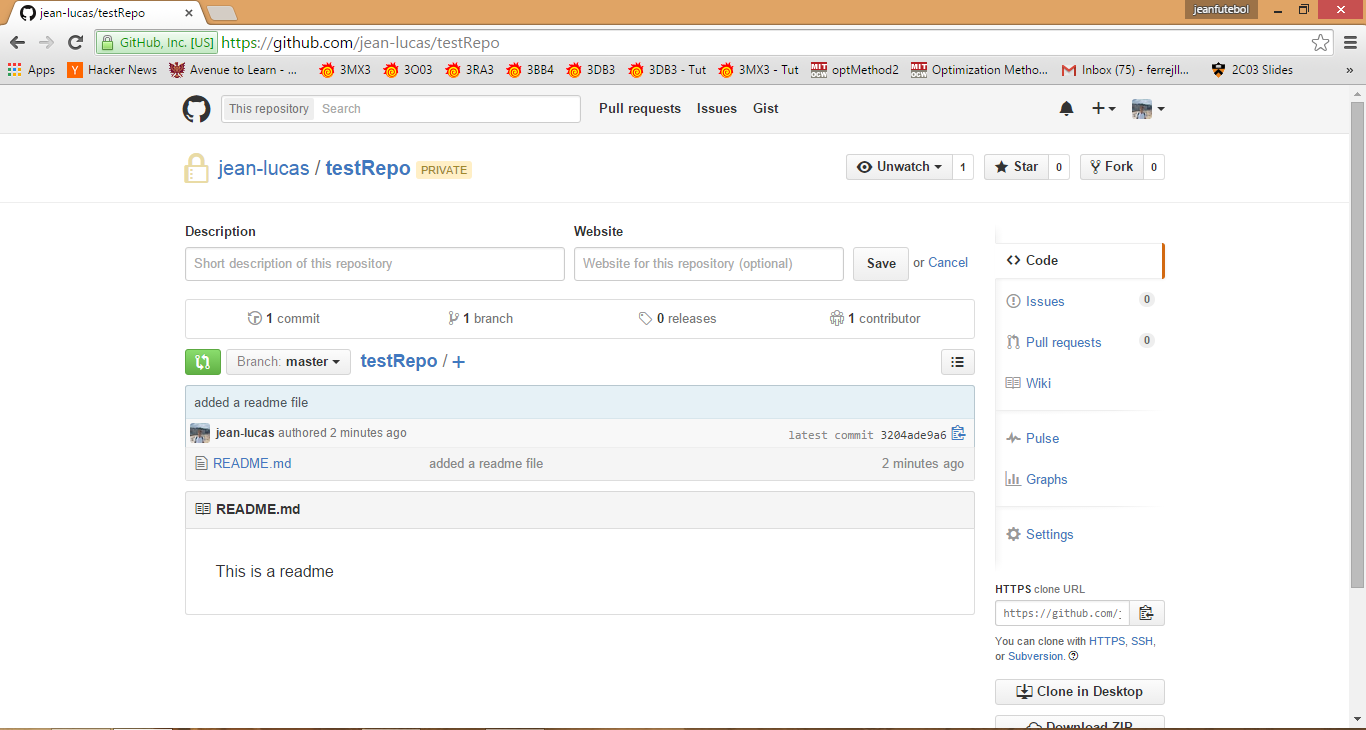
\includegraphics[width=\textwidth]{Capture3.PNG}}
  \caption{Uses Relation}
  \end{figure}


\section{Schedule}

\subsection{Pert Chart}


  \begin{figure}[H]
  \centerline{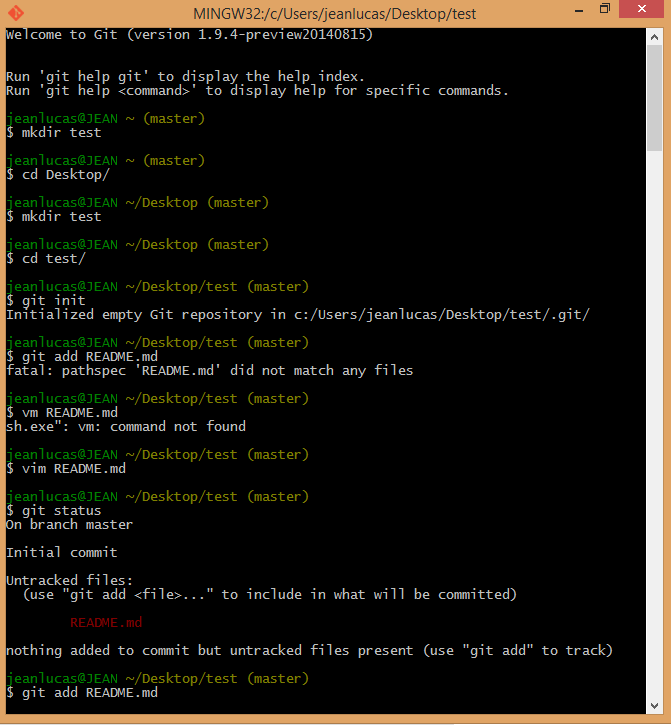
\includegraphics[width=\textwidth]{Capture.PNG}}
  \caption{Pert Chart}
  \end{figure}

\subsection{Gantt Chart}

  \begin{figure}[H]
  \centerline{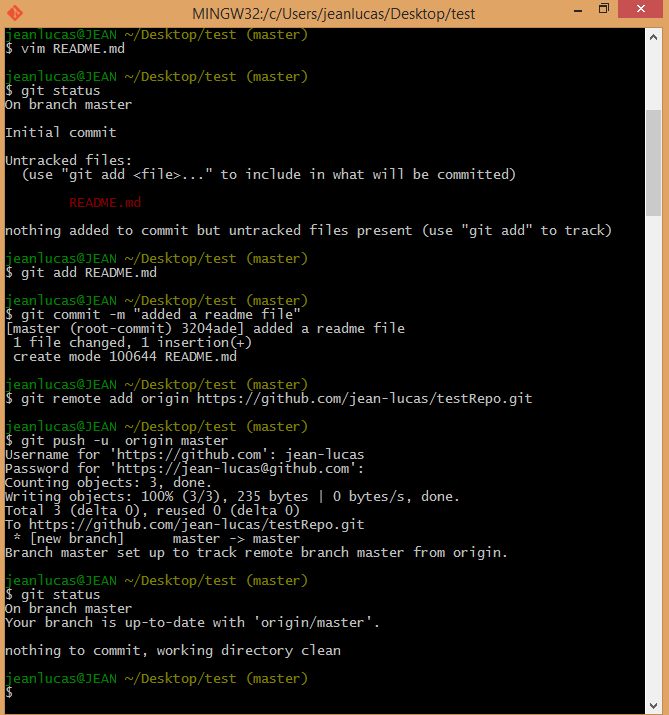
\includegraphics[width=\textwidth]{Capture2.PNG}}
  \caption{Gantt Chart}
  \end{figure}



 \section{\textcolor{red}{MIS for JScrypt}}

 \subsection{\textcolor{red}{Methods}}

\textcolor{red}{\textbf{compareKey(cleanKey, hashKey)}}

\noindent Encrypts the string `cleanKey' and compares to see if the cleanKey is the same as hashKey after the encryption process.

\noindent\textbf{Parameters:}

\begin{table}[H]
\centering
\label{tab:table3}
      \begin{tabular}{ | p{4cm} | p{4cm} | p{9cm} | }
        \hline
            \textbf{Name} & \textbf{Type} & \textbf{Description} \\
        \hline
          cleanKey & string & plain text string that needs to be compared with hashKey  \\
        \hline
          hashKey & string & hashed string generated by the program which consists of version, number of rounds, salt, and encrypted key. \\
       \hline
      \end{tabular}
  \end{table}

Source: JScrypt.js, line 151 \\

\noindent\textbf{\textcolor{red}{generateRandomSalt(rounds)}} \\
\noindent Generates a random padded string of length 24, which is used for hashing the key. This string includes padding which will later be removed before hashing the key.

\noindent\textbf{Parameters:}
\begin{table}[H]
\centering
\label{tab:table4}
      \begin{tabular}{ | p{4cm} | p{4cm} | p{9cm} | }
        \hline
            \textbf{Name} & \textbf{Type} & \textbf{Description} \\
        \hline
          rounds & integer & Number of times the key is hashed.  \\
       \hline
      \end{tabular}
  \end{table}
Source: JScrypt.js, line 41 \\


\noindent\textbf{\textcolor{red}{getComponents(hashKey)}} \\

A String can go through a series of rounds to become hashed and finding the number of rounds in the components gives us the knowledge required to compare a string of plaintext to a hashed string.

\noindent\textbf{Parameters:}
\begin{table}[H]
\centering
\label{tab:table2}
      \begin{tabular}{ | p{4cm} | p{4cm} | p{9cm} | }
        \hline
            \textbf{Name} & \textbf{Type} & \textbf{Description} \\
        \hline
          hashKey & string & string generated by the encryption process with information containing the version, number of rounds, salt, and encrypted key.  \\
       \hline
      \end{tabular}
  \end{table}
Source: Jscrypt.js, line 209 \\

\noindent\textbf{\textcolor{red}{hashKey(rounds, key)}} \\

\noindent Generates the hash string(refer to section 3.4) that will be stored in the applications database. This is the only function that a user of the project will be required to call in order to hash a string to encrypt information.

\begin{table}[H]
\centering
\label{tab:table5}
      \begin{tabular}{ | p{4cm} | p{4cm} | p{9cm} | }
        \hline
            \textbf{Name} & \textbf{Type} & \textbf{Description} \\
        \hline
          rounds & integer & integer input from 6 to 31  \\
        \hline
          key & string & string input of length 1 to 56 characters \\
       \hline
      \end{tabular}
  \end{table}

  Source: JScrypt.js, line 78\\


\section{\textcolor{red}{MIS for eksBlowfish}}

\subsection{\textcolor{red}{eksblowfish}}

\noindent\textcolor{red}{eksBlowfish implementation}

\noindent\textbf{Properties}:

\begin{table}[H]
\centering
\label{tab:table6}
      \begin{tabular}{ | p{4cm} | p{4cm} | p{9cm} | }
        \hline
            \textbf{Name} & \textbf{Type} & \textbf{Description} \\
        \hline
          keyExpansion & function & Sets up the encryption environment with the given key by setting up the P\_arrays and the S\_boxes with hexadecimal values of the key  \\
        \hline
          feistel\_cipher & function & The heart of the encryption. Runs through a feistel network of $2^(number of rounds)$ times. At each iteration, the P\_arrays and S\_boxes are updated according to the salt and the key.  \\
        \hline
          feistal\_F & function & Helper function of the Feistel\_cipher \\
       \hline
      \end{tabular}
Source: eksBlowfish.js, line 15
  \end{table}





\end{document}
